\documentclass[border=10pt]{standalone}
\usepackage[svgnames]{xcolor}
\usepackage{amsmath}
\usepackage{pgfplots}
\pgfplotsset{compat=newest}
\usepackage[sfdefault]{FiraSans}
\usepackage{FiraMono}
\renewcommand*\familydefault{\sfdefault}
\begin{document}
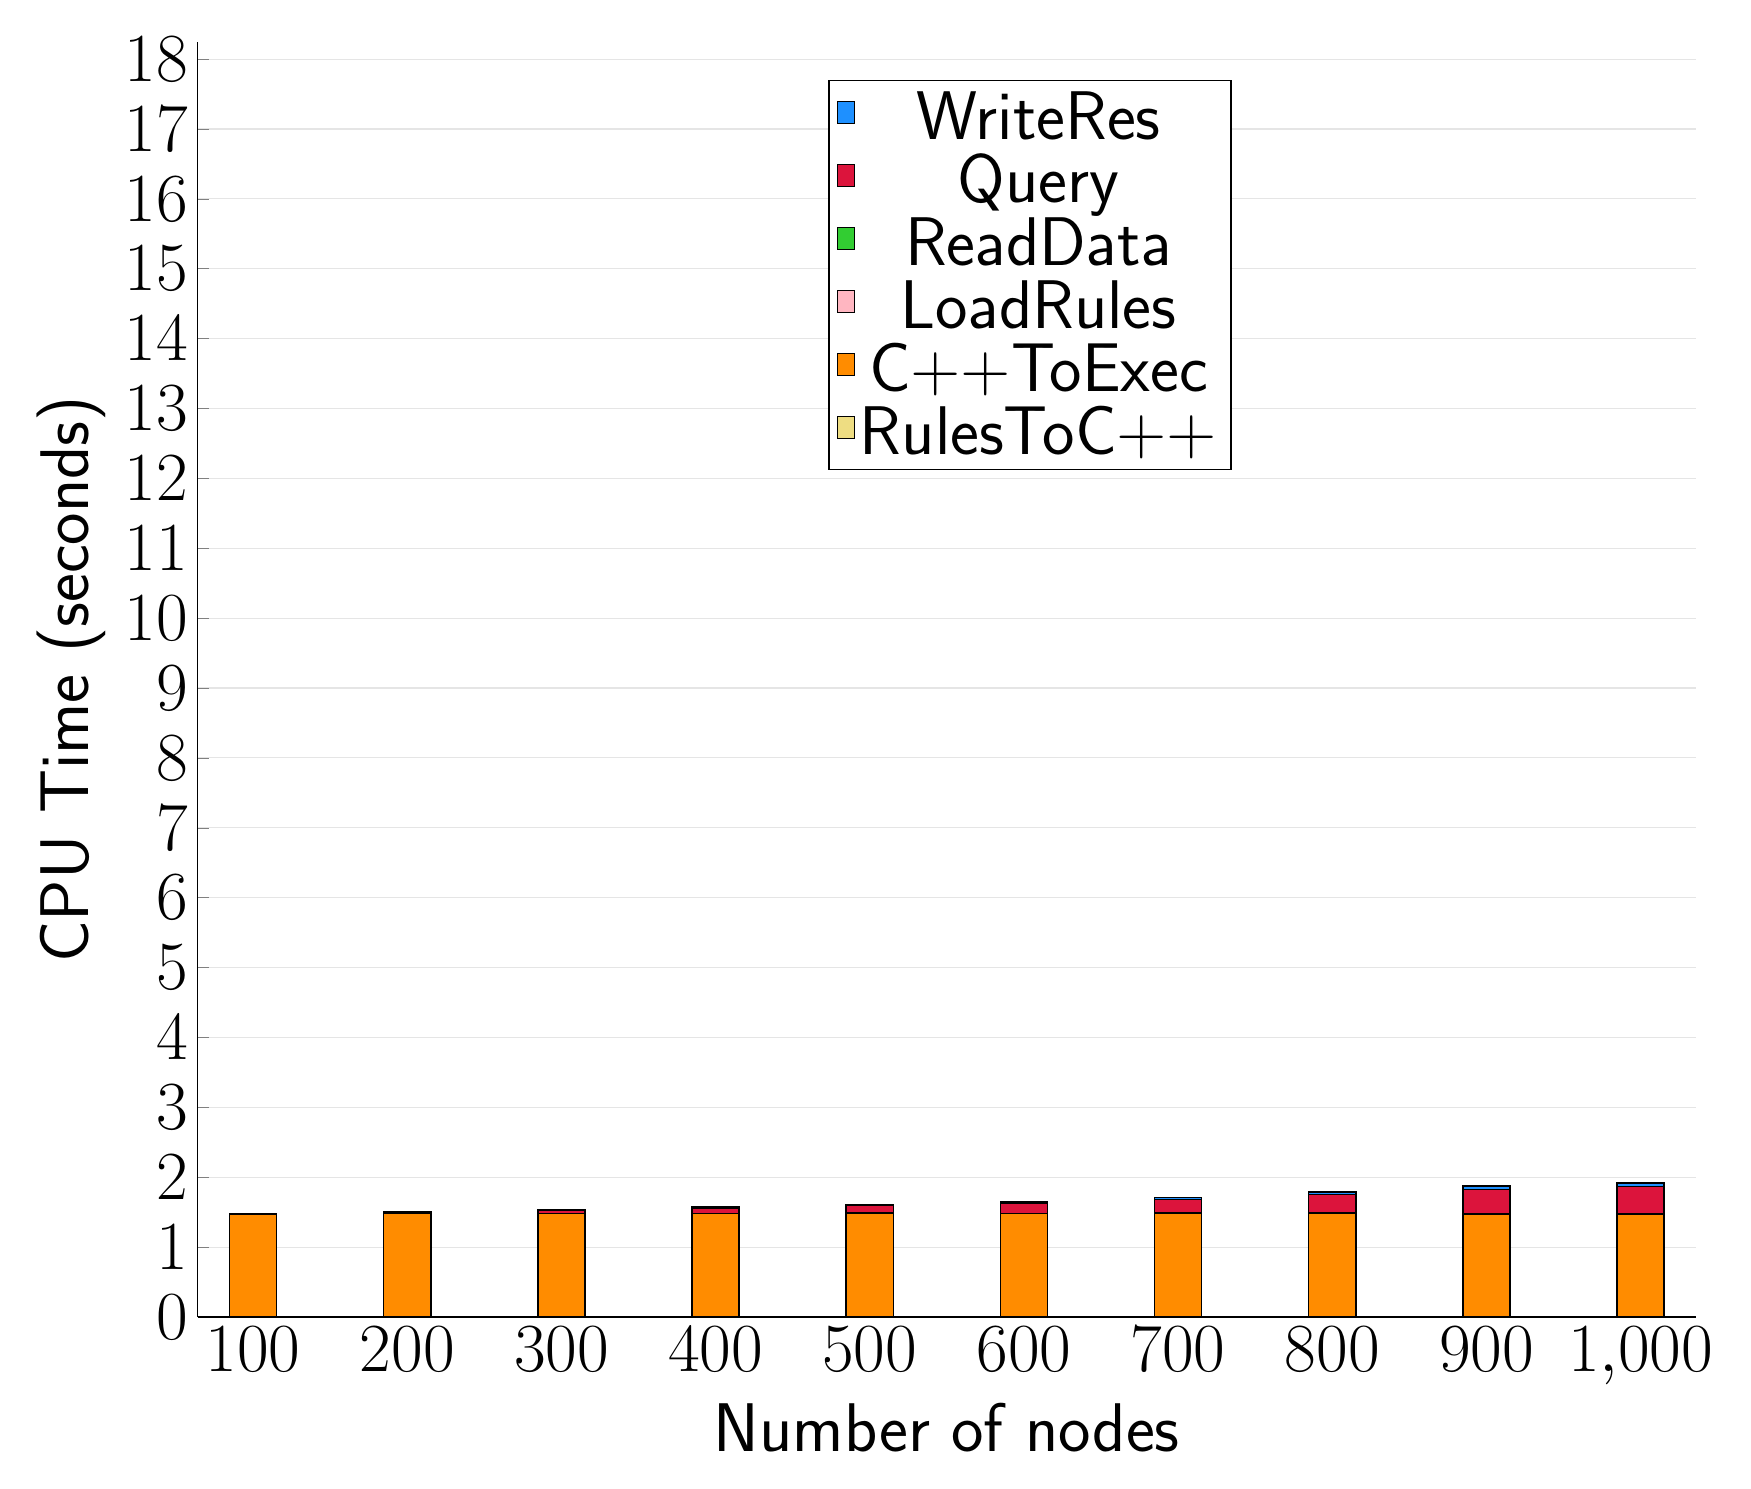
\begin{tikzpicture}
\begin{axis}[
   ybar stacked,
   width=1.7\textwidth,
   bar width=0.6cm,
   ymajorgrids, tick align=inside,
   major grid style={draw=gray!20},
   xtick=data,
   ymin=0, ymax=18.250040000000002,
   axis x line*=bottom,
   axis y line*=left,
   enlarge x limits=0.04,
   legend style={
       at={(0.69, 0.97)},
       anchor=north east,
       legend columns=1,
       font=\Huge,
   },
   ylabel={CPU Time (seconds)},
   xlabel={Number of nodes},
   label style={font=\Huge},
   tick label style={font=\Huge},
]
\addlegendimage{fill=DodgerBlue, draw=black, line width=0.2pt}
\addlegendentry{WriteRes}
\addlegendimage{fill=Crimson, draw=black, line width=0.2pt}
\addlegendentry{Query}
\addlegendimage{fill=LimeGreen, draw=black, line width=0.2pt}
\addlegendentry{ReadData}
\addlegendimage{fill=LightPink, draw=black, line width=0.2pt}
\addlegendentry{LoadRules}
\addlegendimage{fill=DarkOrange, draw=black, line width=0.2pt}
\addlegendentry{C++ToExec}
\addlegendimage{fill=LightGoldenrod, draw=black, line width=0.2pt}
\addlegendentry{RulesToC++}
\addplot +[fill=LightGoldenrod, draw=black, line width=0.55pt] coordinates {
(100, 0.0)
(200, 0.008000000000000002)
(300, 0.004000000000000001)
(400, 0.004000000000000001)
(500, 0.004000000000000001)
(600, 0.006000000000000001)
(700, 0.0020000000000000005)
(800, 0.008000000000000002)
(900, 0.004000000000000001)
(1000, 0.0020000000000000005)
};
\addplot +[fill=DarkOrange, draw=black, line width=0.55pt] coordinates {
(100, 1.472)
(200, 1.47)
(300, 1.4759999999999998)
(400, 1.4739999999999998)
(500, 1.48)
(600, 1.474)
(700, 1.4780000000000002)
(800, 1.476)
(900, 1.472)
(1000, 1.472)
};
\addplot +[fill=LightPink, draw=black, line width=0.55pt] coordinates {
(100, 0.0001672)
(200, 0.00016900000000000002)
(300, 0.00016059999999999997)
(400, 0.0001746)
(500, 0.0001626)
(600, 0.0001392)
(700, 0.00016920000000000002)
(800, 0.0001694)
(900, 0.0001724)
(1000, 0.00016480000000000002)
};
\addplot +[fill=LimeGreen, draw=black, line width=0.55pt] coordinates {
(100, 0.00114)
(200, 0.0017106)
(300, 0.0025714)
(400, 0.0033390000000000004)
(500, 0.003970800000000001)
(600, 0.0042236)
(700, 0.005370000000000001)
(800, 0.005682)
(900, 0.006513200000000001)
(1000, 0.006569)
};
\addplot +[fill=Crimson, draw=black, line width=0.55pt] coordinates {
(100, 0.008927000000000001)
(200, 0.026006400000000002)
(300, 0.0496684)
(400, 0.0814118)
(500, 0.1106984)
(600, 0.1470208)
(700, 0.1990556)
(800, 0.2616562)
(900, 0.34357899999999997)
(1000, 0.3881326)
};
\addplot +[fill=DodgerBlue, draw=black, line width=0.55pt] coordinates {
(100, 0.0016526)
(200, 0.0036851999999999996)
(300, 0.0061098)
(400, 0.0095458)
(500, 0.013808399999999998)
(600, 0.0193574)
(700, 0.026336)
(800, 0.035109)
(900, 0.046283200000000004)
(1000, 0.0522462)
};
\end{axis}
\end{tikzpicture}

\end{document}
